%!TEX root=../document.tex

\section{Aufbau}
Der USART Adapter muss zusätzlich mit dem Microboard an einem USB-Port hängen. Der Adapter steckt dann mit dem \textbf{weißen} Port an \textbf{PA9} und \textbf{gelb} an \textbf{PA10}:

\begin{minipage}{\linewidth}
	\centering
	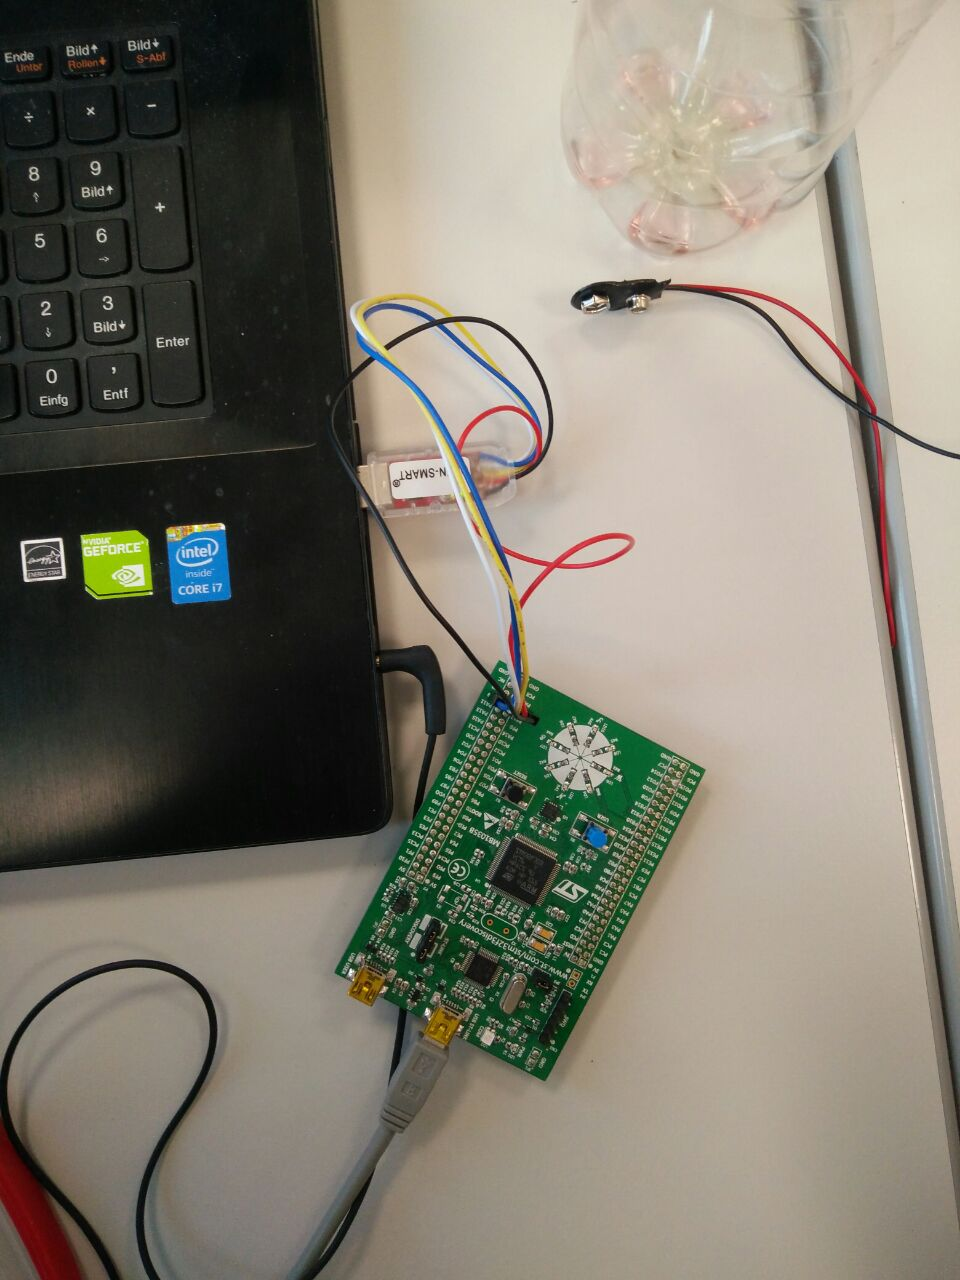
\includegraphics[width=0.8\linewidth]{images/aufbau}
	\figcaption{Aufbau mit dem Adapter und dem Microboard}
\end{minipage}


\section{Daten generieren auf dem Board}
Der nächste Schritt war es nun, ein Programm in C zu schreiben, welches die Daten, welche in der Grundkompetenz in \verb|DataSimulator.java| simuliert wurden, vom Board generieren zu lassen. 

\subsection{Projekt erstellen}
Dazu wurde zuerst ein neues Projekt in der workbench angelegt, wobei zu beachten ist, dass in der neueren Version der workbench die HAL Library nun in jedem Projekt einzeln anzulegen ist und es nicht mehr möglich ist sie als einzelnes Projekt im Workspace liegen zu haben.

\subsection{Konstanten}
Die Parameter welche beim \verb|DataSimulator.java| beim initialisieren angegeben wurden, werden hier nun als globale Konstanten angelegt:

\begin{lstlisting}[language=C]
double initialFrequency = 1;
double deltaFrequency = 0.015;
double valuesPerTimeUnit = 100;
double maxFrequency = 5;
double minFrequency = 0.5;
\end{lstlisting}

\subsection{Port für USART konfigurieren}
Der nächste Schritt war es nun, den Port bzw. die einzelnen Pins für den USART zu initialisieren. Wie schon im Aufbau erwähnt, wurde sich hier für die Pins \textbf{10} und \textbf{9} am Port \textbf{A} entschieden:

\begin{lstlisting}[language=C]
void USART1_GPIO_Configuration(void) {
	GPIO_InitTypeDef GPIO_InitStruct;
	__HAL_RCC_GPIOA_CLK_ENABLE();
	GPIO_InitStruct.Pin = GPIO_PIN_9 | GPIO_PIN_10;
	GPIO_InitStruct.Mode = GPIO_MODE_AF_PP;
	GPIO_InitStruct.Pull = GPIO_PULLUP;
	GPIO_InitStruct.Speed = GPIO_SPEED_FREQ_HIGH;
	GPIO_InitStruct.Alternate = GPIO_AF7_USART1;
	HAL_GPIO_Init(GPIOA, &GPIO_InitStruct);
}
\end{lstlisting}

\subsection{USART konfigurieren}
Dafür wurde neben den Konstanten auch noch eine globale Variable angelegt, namens \verb|UartHandle| vom Typen \verb|UART_HandleTypeDef|.

Als Baudrate, also die Rate wie schnell die Daten ''refreshed'' werden, habe ich das 4. Fache der seriellen Schnittstelle des USB Adapters ausgewählt. Dies konnte ausgelesen werden mit:

\begin{lstlisting}[language=bash]
stty -F /dev/ttyUSB0
\end{lstlisting}

Und lieferte Folgendes Ergebnis

\begin{lstlisting}[language=bash]
speed 9600 baud; line = 0;
-brkint -imaxbel
\end{lstlisting}

Also wurde für die Baudrate \textbf{38400} verwendet, um eine flüssigere Animation zu gestalten:

\begin{lstlisting}[language=c]
void USART1_Configuration(void) {
	USART1_GPIO_Configuration();
	__HAL_RCC_USART1_CLK_ENABLE();
	UartHandle.Instance = USART1;
	UartHandle.Init.BaudRate = 38400;
	UartHandle.Init.WordLength = UART_WORDLENGTH_8B;
	UartHandle.Init.StopBits = UART_STOPBITS_1;
	UartHandle.Init.Parity = UART_PARITY_NONE;
	UartHandle.Init.HwFlowCtl = UART_HWCONTROL_NONE;
	UartHandle.Init.Mode = UART_MODE_TX_RX;
	HAL_UART_Init(&UartHandle);
}
\end{lstlisting}

\subsection{Main Funktion schreiben}
Zuerst werden alle Konfigurationsfunktionen aufgerufen:

\begin{lstlisting}[language=C]
USART1_GPIO_Configuration();
HAL_Init();
USART1_Configuration();
\end{lstlisting}

Und danach werden alle Variablen für die Datengenerierung initialisiert:

\begin{lstlisting}[language=C]
char str1[100];
double actualFrequency = initialFrequency;
double actDeltaFrequency = deltaFrequency;
int values[100];
double waveTime = 0;
\end{lstlisting}

Danach beginnt die while-True Schleife, um die Daten stetig an das Board zu senden:
\begin{lstlisting}[language=C]
for(;;) {
	// Zuerst wird 100 mal iteriert, weil jede Sinus Kurve 100 Werte haben soll
	for (int i=0;i<100;i++) {
		// Es werden die Werte generiert fuer die momentane Frequenz und WaveTime
		values[i] = (int)(10000*sin(waveTime));
		// WaveTime wird angepasst
		waveTime = waveTime + 2*M_PI*actualFrequency/100;
		if (waveTime > 2*M_PI) {
		waveTime = waveTime - 2*M_PI;
		}
	}
	// Frequenzen wird angepasst
	actualFrequency = actualFrequency * (1+actDeltaFrequency);
	if (actualFrequency>5) {
		actDeltaFrequency = -0.015;
	}
	if (actualFrequency<minFrequency) {
		actDeltaFrequency = 0.015;
	}

	// Daten werden an UART weitergeleitet
	for (int var = 0; var < 100; ++var) {
		if(var == 0){
			sprintf(str1, "$%d", values[var]);
			HAL_UART_Transmit(&UartHandle, (uint8_t *)str1, strlen(str1), 5000);
		}else if(var == 99){
			sprintf(str1, ",%d\n", values[var]);
			HAL_UART_Transmit(&UartHandle, (uint8_t *)str1, strlen(str1), 5000);
		}else{
			sprintf(str1, ",%d", values[var]);
			HAL_UART_Transmit(&UartHandle, (uint8_t *)str1, strlen(str1), 5000);
		}
	}
}
\end{lstlisting}

\section{Daten auslesen vom dem Board}
Anstatt die Daten nun in \verb|DataSimulator.java| zu simulieren, werden sie in \verb|DataGenerator.java| vom  Board ausgelesen.

\subsection{Attribute}
Zuerst werden die nötigen Attribute angelegt:
\begin{lstlisting}[language=Java]
static SerialPort sp;
static ArrayList<String> data = new ArrayList<String>();
static DataBuffer db;
\end{lstlisting}

Als nächstes werden im Konstruktor alle relevanten Objekte und Variablen initialisiert, und der Parameter übernommen:

\begin{lstlisting}[language=Java]
public DataGenerator(DataBuffer db) {
	this.db = db;
	
	// Da ich in Linux arbeite, musste ich zuerst den Portnamen ausgeben, damit ich erkenne wie dieser heisst
	System.out.println(SerialPortList.getPortNames()[0]);
	// Das Ergebnis war /dev/ttyUSB0
	this.sp = new SerialPort("/dev/ttyUSB0");
	
	try {
		// Hilfe von Johannes Bishara
		this.sp.openPort();
		this.sp.setParams(38400, 8, 1, 0);
		int mask = SerialPort.MASK_RXCHAR + SerialPort.MASK_CTS + SerialPort.MASK_DSR;
		this.sp.setEventsMask(mask);
		this.sp.addEventListener(new SerialPortReader());
	} catch (SerialPortException ex) {
		// Bei einer Exception einen Fehler ausgeben
		System.out.println(ex);
}
\end{lstlisting}

\subsection{SerialPortEventListener implementieren}
Als nächstes wird der SerialPortEventListener implementiert:

\begin{lstlisting}[language=Java]
// Methode wird ueberladen
public void serialEvent(SerialPortEvent event) {
try {
String getdata = sp.readString(event.getEventValue());
String[] parts = getdata.split("\\$");

if (data.size() > 0)
data.set(data.size() - 1, data.get(data.size() - 1) + parts[0]);
for (int i = 1; i < parts.length; i++) {
data.add(parts[i]);
}

String daten = "";
try {
daten = data.get(data.size() - 1);
} catch (ArrayIndexOutOfBoundsException e) {
return;
}

// Aus der Datenliste werden die einzelnen Teile extrahiert mit split
String[] teile = daten.split(",");

// Falls es 100 sind, was vorgegebn ist durch den Generator am Board
if (teile.length == 100) {
// Die Liste welche dann an datenbuffer uebergeben wird
int fertig[] = new int[100];
for (int i = 0; i < fertig.length; i++) {
// Falls ein Teil nicht null ist
if (teile[i] != null) {
// Versuchen den String zu einem Int zu parsen
int d = 0;
try {
d = Integer.parseInt(teile[i].trim());
} catch (NumberFormatException e) {
// do nothing, encoding error
}
fertig[i] = d;
}
}
db.addList(fertig);
}
} catch (SerialPortException ex) {
ex.printStackTrace();
}
}
\end{lstlisting}


\section{Ergebnis}
\begin{minipage}{\linewidth}
	\centering
	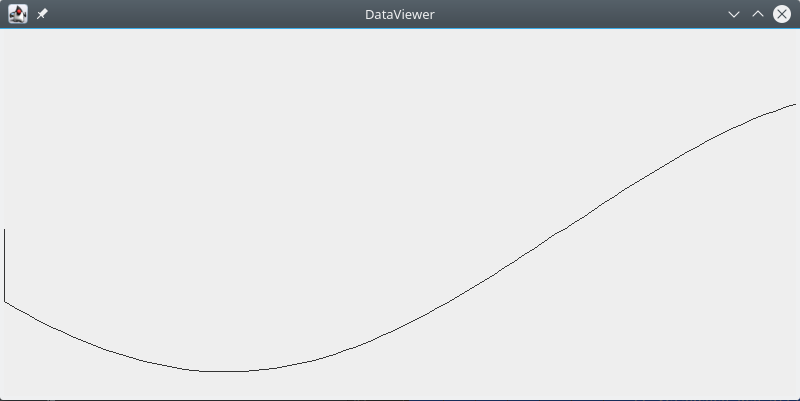
\includegraphics[width=0.8\linewidth]{images/ergebnis}
	\figcaption{Ergebnis}
\end{minipage}